\begin{SCn}

\scnsectionheader{\currentname}

\scnstartsubstruct

\scnheader{Предметная область и онтология решателей задач ostis-систем}
\scnsdmainclasssingle{решатель задач ostis-системы}
\scnsdclass{***}
\scnsdrelation{***}

\scnheader{решатель задач ostis-системы}
\scnrelfromlist{включение}{решатель задач IMS;решатель задач вспомогательной компьютерной системы\\
    \scnaddlevel{1}
    \scnrelfromlist{включение}{решатель задач интерфейса компьютерной системы\\
        \scnaddlevel{1}
        \scnrelfromlist{включение}{решатель задач пользовательского интерфейса компьютерной системы;решатель задач интерфейса компьютерной системы с другими компьютерными системами;решатель задач интерфейса компьютерной системы с окружающей средой}
        \scnaddlevel{-1}
    ;решатель задач подсистемы поддержки проектирования компонентов определенного класса\\
        \scnaddlevel{1}
        \scnrelfromlist{включение}{решатель задач подсистемы поддержки проектирования баз знаний\\
            \scnaddlevel{1}
            \scnrelfrom{включение}{машина повышения качества базы знаний\\
                \scnaddlevel{1}
                \scnrelfromlist{включение}{машина верификации базы знаний\\
                    \scnaddlevel{1}
                    \scnrelfromlist{включение}{машина поиска и устранения некорректностей;машина поиска и устранения неполноты}
                    \scnaddlevel{-1}
                ;машина оптимизации базы знаний;машина выявления и устранения информационного мусора}
                \scnaddlevel{-1}}
            \scnaddlevel{-1}
        ;решатель задач подсистемы поддержки проектирования решателей\\
            \scnaddlevel{1}
            \scnrelfromlist{включение}{решатель задач подсистемы поддержки проектирования программ обработки знаний;решатель задач подсистемы поддержки проектирования агентов обработки знаний}
            \scnaddlevel{-1}
        \scnaddlevel{-1}}
    ;решатель задач подсистемы управления проектирования компьютерных систем и их компонентов}
    \scnaddlevel{-1}
;решатель задач самостоятельной компьютерной системы}

\scnheader{решатель задач ostis-системы}
\scnrelfromlist{включение}{машина информационного поиска\\
    \scnaddlevel{1}
    \scnrelfromlist{включение}{машина информационного поиска информации, удовлетворяющей заданной спецификации;машина информационного поиска информации, не удовлетворяющей заданной спецификации;машина, выявляющая отсутствие информации, удовлетворяющей заданной спецификации}
    \scnaddlevel{-1}
;решатель задач с использованием хранимых программ\\
    \scnaddlevel{1}
    \scnrelfromlist{включение}{интерпретатор нейросетевых моделей;интерпретатор генетических алгоритмов;интерпретатор императивных программ\\
        \scnaddlevel{1}
        \scnrelfromlist{включение}{интерпретатор процедурных программ;интерпретатор объектно-ориентированных программ}
        \scnaddlevel{-1}
    ;интерпретатор декларативных программ\\
        \scnaddlevel{1}
        \scnrelfromlist{включение}{интерпретатор логических программ;интерпретатор функциональных программ}
        \scnaddlevel{-1}}
    \scnaddlevel{-1}
;решатель задач в условиях, когда программа решения не известна\\
    \scnaddlevel{1}
    \scnrelfromlist{включение}{решатель, реализующий поиск решения задачи в глубину;решатель, реализующий поиск решения задачи в ширину;решатель, реализующий метод проб и ошибок;решатель, реализующий метод разбиения задачи на подзадачи;решатель, реализующий метод решения задач по аналогии;решатель, реализующий метод сведения условия задачи к языку логики предикатов первого порядка;машина логического вывода\\
        \scnaddlevel{1}
        \scnrelfromlist{включение}{машина дедуктивного вывода\\
            \scnaddlevel{1}
            \scnrelfromlist{включение}{машина прямого дедуктивного вывода;машина обратного дедуктивного вывода}
            \scnaddlevel{-1}
        ;машина индуктивного вывода;машина абдуктивного вывода;машина нечеткого вывода;машина вывода на основе логики умолчаний;машина темпорального логического вывода}
        \scnaddlevel{-1}}
    \scnaddlevel{-1}}

\scnheader{решатель задач ostis-системы}
\scnrelfromlist{включение}{решатель явно сформулированных задач\\
    \scnaddlevel{1}
    \scnrelfromlist{включение}{машина поиска значений заданного множества величин;машина установления истинности заданного логического высказывания в рамках заданной формальной теории;машина формирования способа решения указанной задачи\\
        \scnaddlevel{1}
        \scnrelfromlist{включение}{машина формирования доказательства заданного высказывания в рамках заданной формальной теории}
        \scnaddlevel{-1}
    ;машина верификации ответа на указанную задачу;машина верификации способа решения указанной задачи\\
        \scnaddlevel{1}
        \scnrelfromlist{включение}{машина верификации доказательства заданного высказывания в рамках заданной формальной теории}
        \scnaddlevel{-1}}
    \scnaddlevel{-1}
;машина классификации сущностей\\
    \scnaddlevel{1}
    \scnrelfromlist{включение}{машина соотнесения сущности с одним из заданного множества классов;машина разделения множества сущностей на классы по заданному множеству признаков}
    \scnaddlevel{-1}
;машина синтеза естественно-языковых текстов;машина анализа естественно-языковых текстов\\
    \scnaddlevel{1}
    \scnrelfromlist{включение}{машина распознавания естественно-языковых текстов;машина верификации естественно-языковых текстов}
    \scnaddlevel{-1}
;машина синтеза сигналов\\
    \scnaddlevel{1}
    \scnrelfrom{включение}{машина синтеза речи}
    \scnaddlevel{-1}
;машина анализа сигналов\\
    \scnaddlevel{1}
    \scnrelfrom{включение}{машина анализа речи\\
        \scnaddlevel{1}
        \scnrelfrom{включение}{машина распознавания речи}
        \scnaddlevel{-1}}
    \scnaddlevel{-1}
;машина обработки мультимедийных данных\\
    \scnaddlevel{1}
    \scnrelfrom{включение}{машина анализа изображений\\
        \scnaddlevel{1}
        \scnrelfrom{включение}{машина машина распознавания изображений}
        \scnaddlevel{-1}}
    \scnaddlevel{-1}}

\scnheader{структура}
\scnsubdividing{sc-конструкция нестандартного вида;sc-конструкция стандартного вида\\
    \scnaddlevel{1}
    \scnsubdividing{одноэлементная sc-конструкция;трехэлементная sc-конструкция;пятиэлементная sc-конструкция}
    \scnaddlevel{-1}}
    
\scnheader{sc-конструкция нестандартного вида}
\scnexplanation{Каждая \textit{sc-конструкция нестандартного вида} состоит из произвольного количества \textit{sc-элементов} произвольного типа.

\begin{figure}[H]
  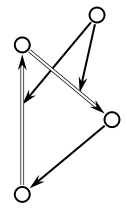
\includegraphics{figures/sd_ps/pic_ps1.png}
\end{figure}}

\scnheader{sc-конструкция стандартного вида}
\scnexplanation{В свою очередь, каждый элемент \textit{\mbox{sc-конструкции} стандартного вида} имеет свою условную строго фиксированную позицию в рамках этой \mbox{sc-конструкции} (первый элемент, второй элемент и т. д.). В зависимости от указанной позиции вводятся дополнительные ограничения на тип соответствующего \textit{sc-элемента}.}

\scnheader{одноэлементная sc-конструкция}
\scnexplanation{Каждая \textit{одноэлементная sc-конструкция} состоит из одного \textit{sc-элемента} произвольного типа.

\begin{figure}[H]
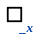
\includegraphics{figures/sd_ps/pic_ps2.png}
\end{figure}}

\scnheader{трехэлементная sc-конструкция}
\scnexplanation{Каждая \textit{трехэлементная sc-конструкция} состоит из трех \textit{sc-элементов}. Второй элемент всегда является \textit{sc-коннектором}, остальные элементы могут быть произвольного типа.

\begin{figure}[H]
  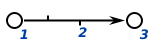
\includegraphics{figures/sd_ps/pic_ps3.png}
\end{figure}}

\scnheader{пятиэлементная sc-конструкция}
\scnexplanation{Каждая \textit{пятиэлементная sc-конструкция} состоит из пяти \textit{sc-элементов}. Второй и четвертый элементы обязательно являются \textit{sc-коннекторами}, остальные элементы могут быть произвольного типа.

\begin{figure}[H]
  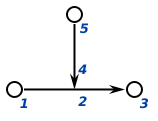
\includegraphics{figures/sd_ps/pic_ps4.png}
\end{figure}}

\scnendstruct \scnendcurrentsectioncomment

\end{SCn}